\section*{Fase 2}

\subsection*{Afgrænsning af baseline-systemet}

Base systemet er det hvor musik bliver distribueret igennem LP plader, CD'er og online tjenester. De vigtigste processer er afgrænset til anskaffelse af råmaterialer til produkt produktion, brug og bortskaffelse.
LP plader er lavet af polyvinylchlorid som kræver udvinding af fossile ressourcer som natur gasser, petroleum og olie. 
Der antages at musik lyttere ejer elektroniske enheder som muliggøre streaming uanset lytnings metode, men uanset lytnings metode antages det også at kræve energi ved brug.
I forlængelse af musik distribution via LP plader, skal afspilningsenheder også produceres og distribueres. 
Når CD'er, LP'er, afspilingsenheder ikke kan bruges længere bortksaffes de ved forbrænding, genbrug og opbevaring på losseplads.
Afspilningsenheder indeholder elektroniske komponenter som derfor bliver bortskaffet via adskillelse og genbrug.
Distribution via streaming kræver produktion, opbevaring, operation og vedligeholdese af servere i eksempelvis et data centre.
Minedrift og udvinding af råstoffer understøtter fremstilling af datacentre med servere, nedkølings anlæg mm.
Minedrift og udvinding af råstoffer støtter også produktionen af afspilingsenheder. 
Operationen og vedligeholdese af datacentre der facilitere musik streaming kræver energi til at holde servere tændt samt temperatur kontrol.
Når servere og køleanlæger afskaffes bliver de afskaffet ved adskillelse og genbrug af materialer eller opbevaring på losseplads.

Det nye system er det hvor musik bliver udelukkende distribueret igennem online streaming tjenester, hvilket ikke resultere i nye processor men udfasningen nogle.
Plader og afspilningsenheder vil ikke længere blive produceret i det nye system, hvilket også medfører at anskaffelse og afskaffelsen ikke længere er muligt.


\begin{figure}[H]
    \centering
    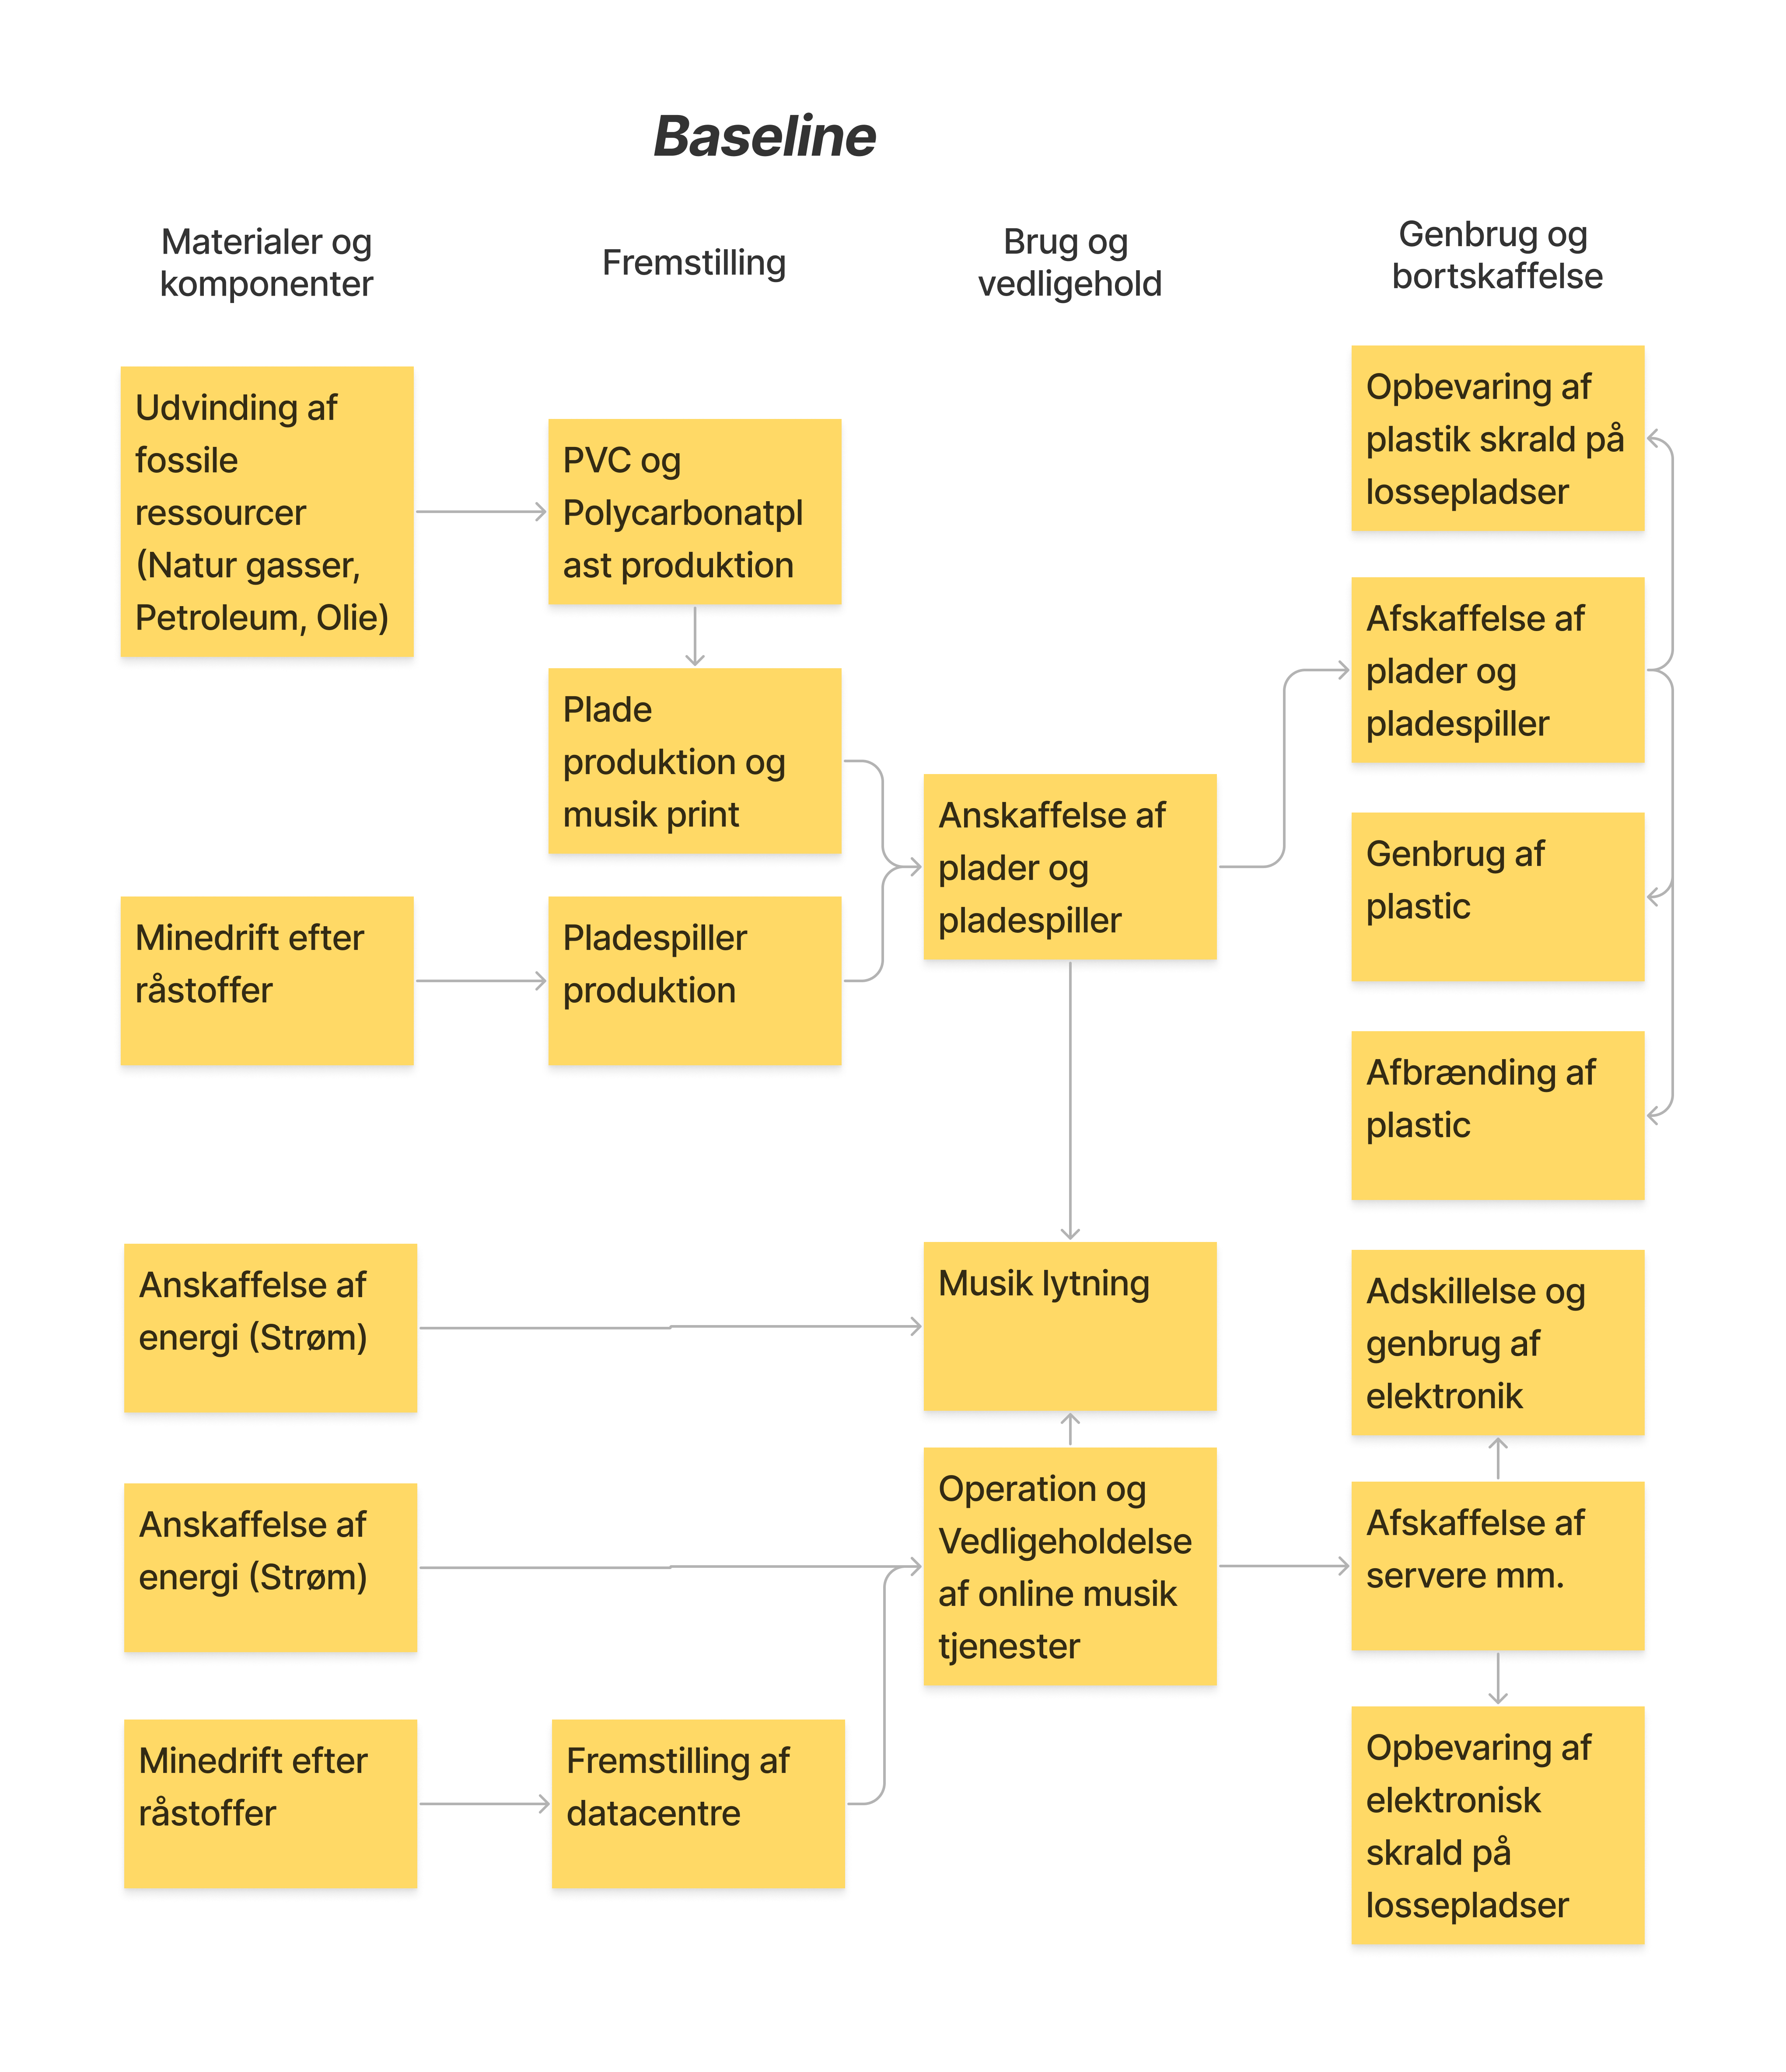
\includegraphics[width=0.5\textwidth]{images/baseline.png}
    \caption{Diagram over det afgrænsede baseline-system}
    \label{fig:baseline}
\end{figure} 


\subsection*{Afgrænsning af det nye system}

\begin{figure}[H]
    \centering
    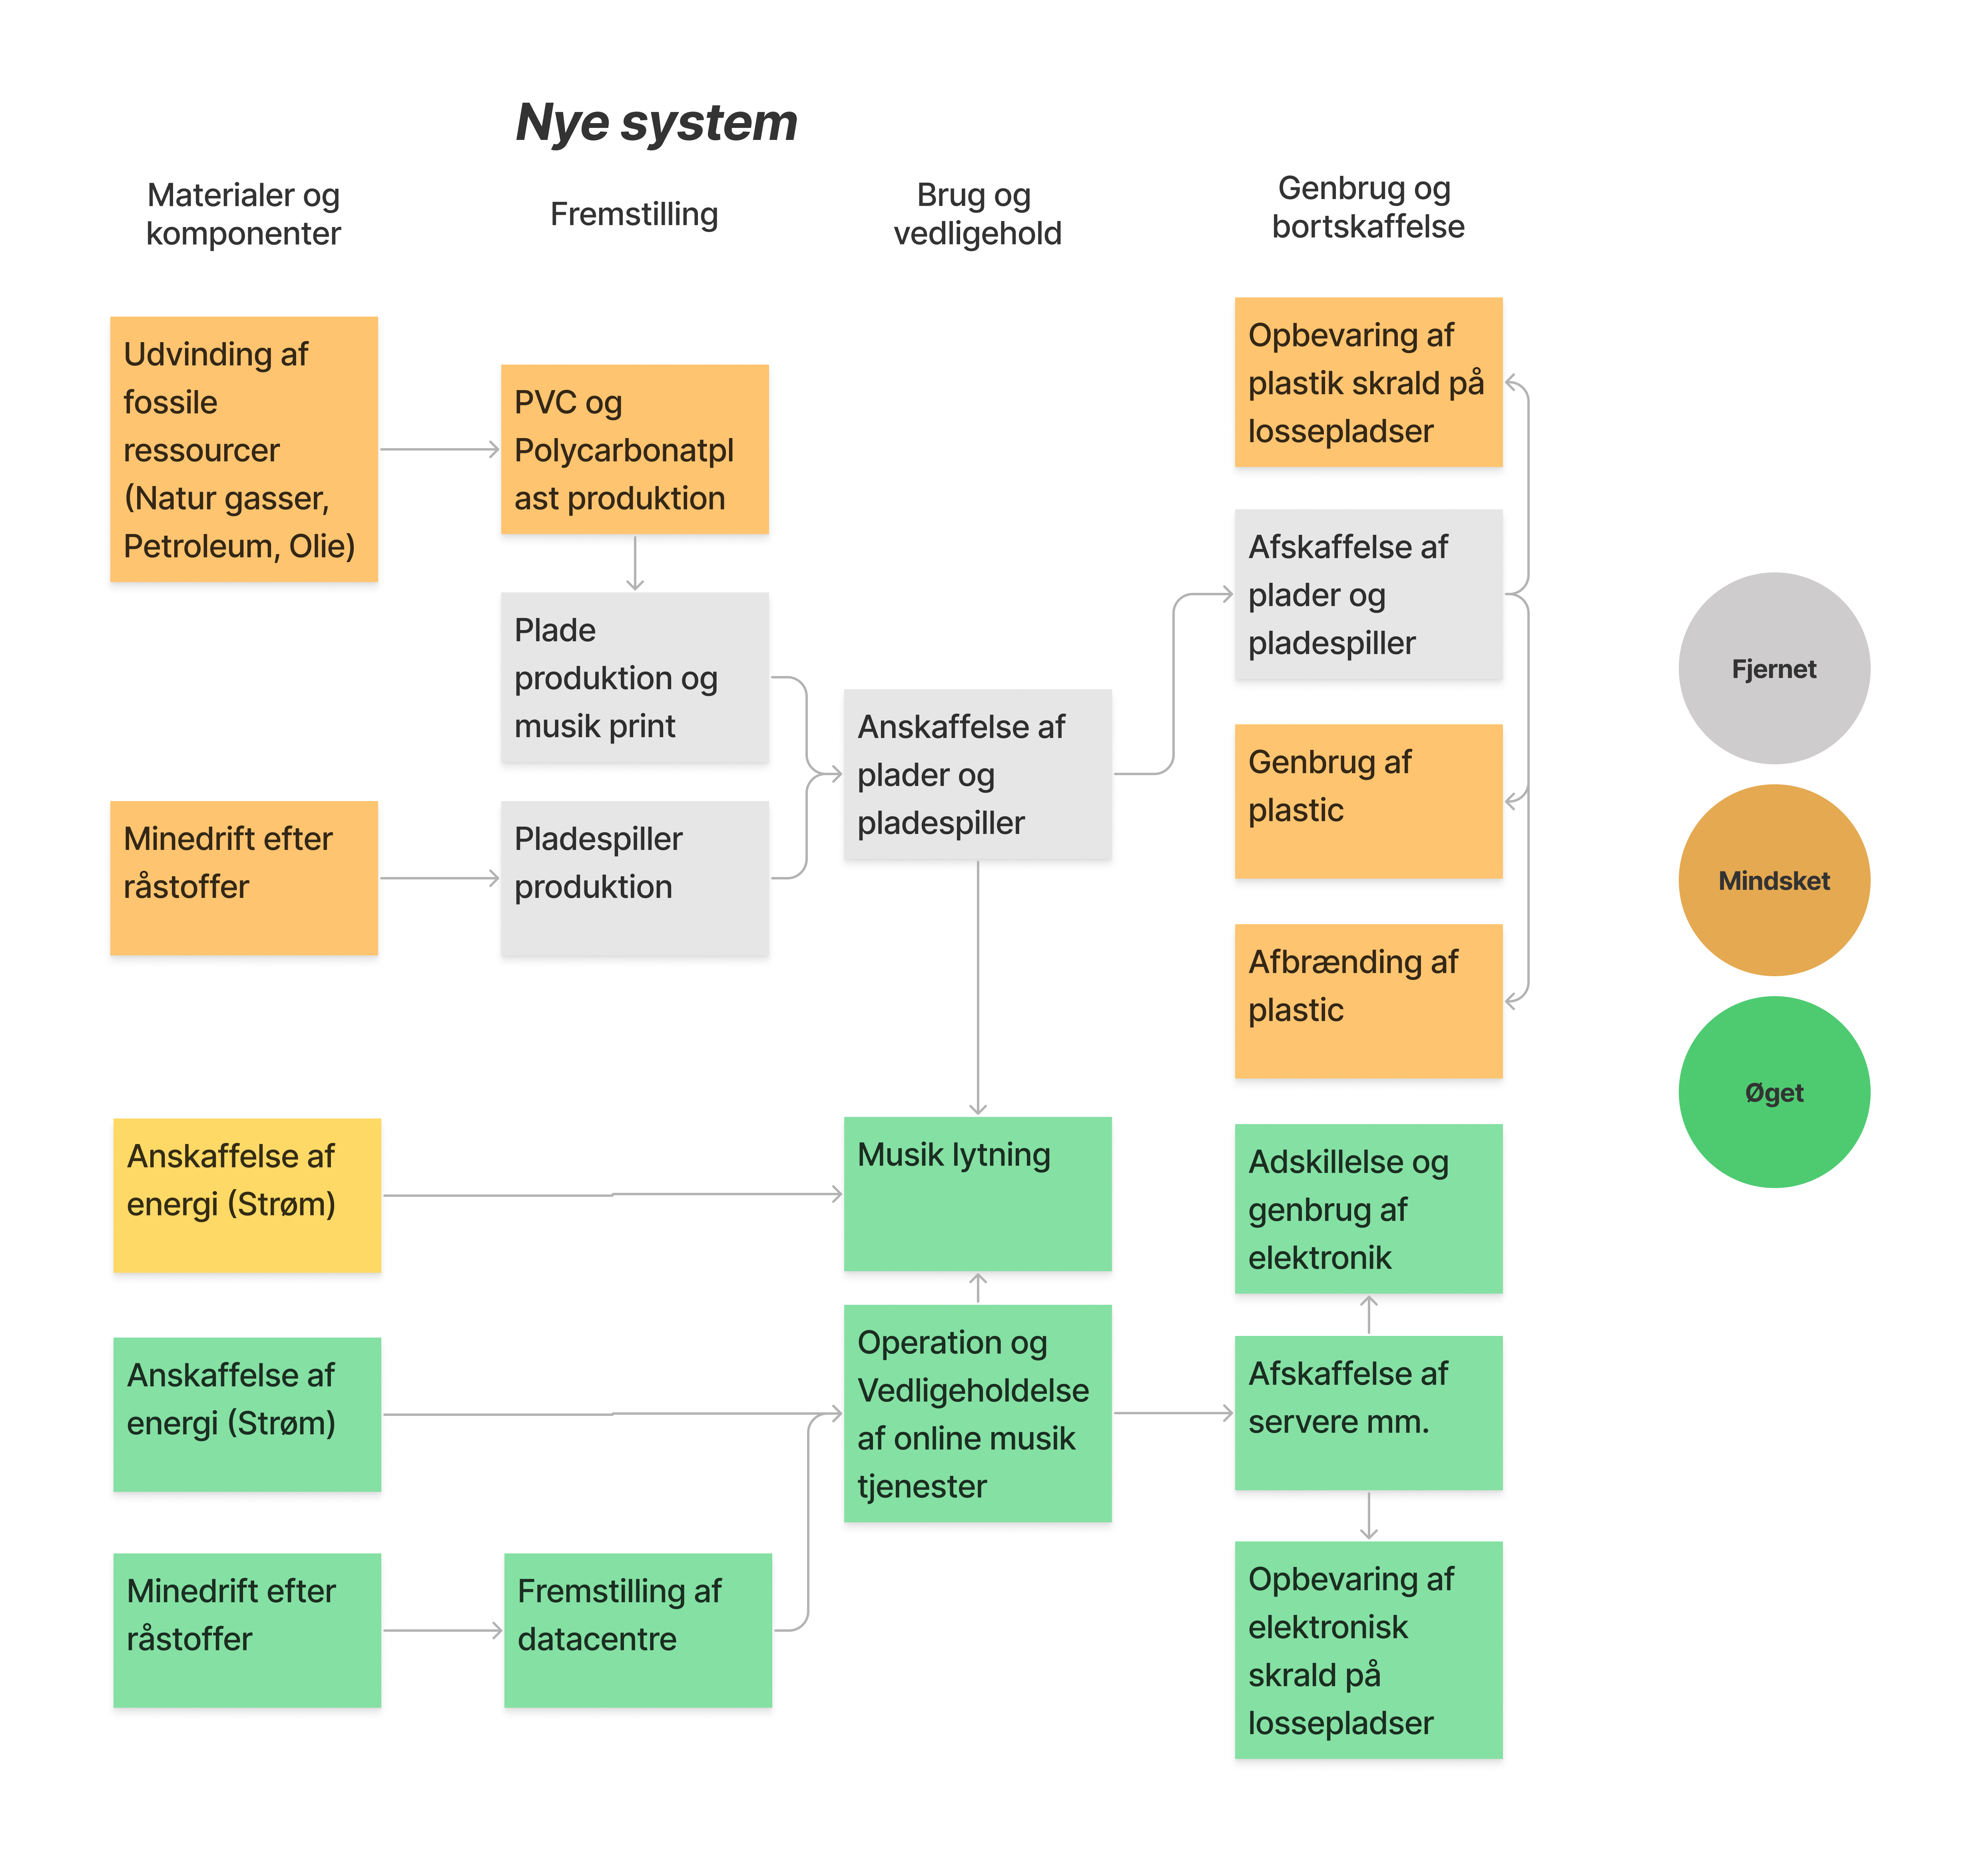
\includegraphics[width=0.7\textwidth]{images/nytsystem.png}
    \caption{Diagram over det afgrænsede nye system}
    \label{fig:nyt}
\end{figure} 

Da plade produktion udfases, vil rå materialer brugt i produktionen ikke længere være i lige så stort behov. 
Den PVC og Polycarbonat der bruges i LP plader og CD'er produktion vil ikke være nødvendigt, hvilket aflaster produktionen af PVC og Polycarbonat.
Ved aflastningen af PVC og Polycarbonat produktion vil den nødvendige mængde af fossile ressourcer også falde, hvilket reducere behovet for udvinding af fossile ressourcer.
Da LP'er og CD'er udfases er det ikke ængere nødvendigt at producere specielle afspilningsenheder og derved minimere behovet for råstoffer.
Med afskaffelsen af LP plader og CD'er vil der naturligvis være mindre af disse plastikker i skrald generation til genbrug eller afbrænding.
Trenden om at musik lytningen er højere ved lytningen via streaming, vil ved udfasningen af LP'er og CD'er resultere i øget musik lytning.
Når musik lytningen udelukkende består af streaming via online musik tjenester, vil belastningen på operationen, vedligeholdesen og skaleringen af servere i datacentrer stige.
Den øget belastning på datacentrer medføre et højere behov for fremstillingen af bedre, flere og nye datacentre.
Med et højere behov for datacentre vil behovet for råmaterialer fra minedrift mm, også øges.
Et kritisk aspect operatinen og vedligeholdesen af servere i datacentrer er temperatur kontrol, og ved en højere belastning vil belastningen på temperatur kontrollen også øges hvilket resultere i højere behov for anskaffelse af energi.  
Da der vil være flere servere og kølinganlæger i brug, vil afskaffelsen af disse også stige.
